%%%%%%%%%%%%%%%%%%%%%%%%%%%%%%%%%%%%%%%%%
%
% (c) 2018 by Jennifer Laaser
%
% This work is licensed under the Creative Commons Attribution-NonCommercial-ShareAlike 4.0 International License. To view a copy of this license, visit http://creativecommons.org/licenses/by-nc-sa/4.0/ or send a letter to Creative Commons, PO Box 1866, Mountain View, CA 94042, USA.
%
% The current source for these materials is accessible on Github: https://github.com/jlaaser/quantum-exercises
%
%%%%%%%%%%%%%%%%%%%%%%%%%%%%%%%%%%%%%%%%%

\section*{Tunneling\sectionmark{Exercise: Tunneling}}

	Consider a particle incident ``from the left'' on the following potential barrier, with the particle's energy less than the barrier height, e.g. $0<E<V_0$:
		
			\vspace{0.1in}
			\centerline{
				\begin{minipage}{0.5\textwidth}
					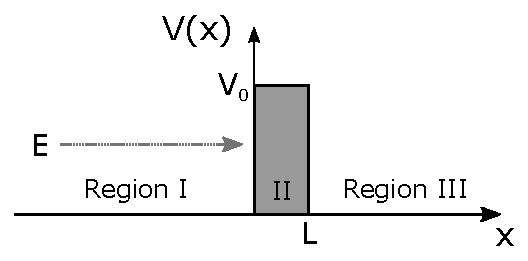
\includegraphics[width=\textwidth]{includes/tunneling-FIGURES/tunneling.pdf}
				\end{minipage}
				\begin{minipage}{0.3\textwidth}
					\begin{equation}
				 		V(x)=\begin{cases}0 & x<0 \\ V_0 & 0 \leq x \leq L \\ 0 & x>L \end{cases} \nonumber
					\end{equation}
				\end{minipage}
		}\vspace{-0.1in}

	\begin{questions}
	
		\question What are the general solutions for the wavefunction in each region? Make sure to include any appropriate coefficients and substitute in the correct value of $V$ in each region.
		
			\begin{minipage}{0.1\textwidth}.
			\end{minipage}
			\begin{minipage}{0.4\textwidth}
			\begingroup
\addtolength{\jot}{1em}
			\begin{align*}
				\Psi_I(x) = \answerbox{150}\\
				\Psi_{II}(x) = \answerbox{150}\\
				\Psi_{III}(x) = \answerbox{150}
			\end{align*}
			\endgroup
			\end{minipage}
			\begin{minipage}{0.4\textwidth}
			\begingroup
\addtolength{\jot}{1em}
			\begin{align*}
				k = \answerboxtall{60}\\
				\kappa = \answerboxtall{60}
			\end{align*}
			\endgroup
			\end{minipage}
			
			\vspace{0.1in}
		\question What are the boundary conditions necessary for...
		
			\begin{parts}
				\part ... the \emph{wavefunction} to be continuous at $x=0$ and $x=L$?
				
					%\emph{(Note: you don't need to plug anything into the wavefunctions; it's sufficient to write your answers in the form of $\Psi_I(x_0) = \Psi_{II}(x_0)$, etc.)}
				
					\begin{solution}[1.5in]
					\end{solution}
				
				\part ... the \emph{first derivative} of the wavefunction  to be continuous at $x=0$ and $x=L$?
				
					\begin{solution}[1.3in]
					\end{solution}
				
				\contdnewpg 
				
				\part ... the particle to be incident only from the left?
				
					\begin{solution}[1.5in]
					\end{solution}
				
				%\part ... ``arbitrary'' normalization?
				
				%	\begin{solution}[1.5in]
				%	\end{solution}
			\end{parts}
		
		\question What ratio would you calculate if you wanted to find the probability that the particle is transmitted through the barrier (e.g. the tunneling probability)?
				
					\begin{solution}[1.5in]
					\end{solution}
		
		\question If you do all the algebra, you will find that the tunneling probability for a tall, thin barrier is approximately
			\begin{equation*}
				T = \frac{16E(V_0-E)}{V_0^2} e^{-2\sqrt{\frac{2m(V_0-E)}{\hbar^2}}L}
			\end{equation*}
			
			What do you predict would happen to to the tunneling probability if...
			\begin{parts}
				\part ... you increased the particle's mass?
				
					\begin{solution}[1.5in]
					\end{solution}
				
				\part ... you decreased the barrier width?
				
					\begin{solution}[1.5in]
					\end{solution}
			\end{parts}
	\end{questions}	
	